\documentclass{article}

\usepackage[utf8]{inputenc}
\usepackage[T1]{fontenc}
\usepackage{amsmath}
\usepackage{amsfonts}
\usepackage{amssymb}
\usepackage[version=4]{mhchem}
\usepackage{stmaryrd}
\usepackage{bbold}
\usepackage{graphicx}
\usepackage{adjustbox}
\usepackage{hyperref}  % For clickable links in TOC
\usepackage{tocloft}   % For TOC formatting
\usepackage{geometry}  % For margins
\usepackage{titlesec}  % For section formatting
\usepackage{fancyhdr}
\usepackage{subcaption}  
\usepackage{footmisc}
\usepackage{booktabs}
\usepackage{siunitx}
\usepackage{float}
\usepackage{tikz} 
\usepackage{caption}  
\usepackage{geometry}[margin=1in]
\usepackage{threeparttable} 
\usepackage{sectsty}  
\usepackage{titling}  
\usepackage{lmodern}  
\usepackage{setspace} 


% Retrieves visuals 
% visuals

\usepackage[most]{tcolorbox}

% equation system NSS blue
\newtcolorbox{Recapbox1}[1][]{%
  enhanced,
  colback=blue!2!white,
  colframe=blue!75!black,,
  arc=4mm,                % rounded corners
  fonttitle=\bfseries,
  title={RECAP : Choice variables},
  center title,
  #1
}
\newtcolorbox{Recapbox2}[1][]{%
  enhanced,
  colback=green!2!white,
  colframe=green!75!black,,
  arc=4mm,                % rounded corners
  fonttitle=\bfseries,
  title={RECAP : Parameters},
  center title,
  #1
}

\newtcolorbox{Recapbox3}[1][]{%
  enhanced,
  colback=red!2!white,
  colframe=red!75!black,,
  arc=4mm,                % rounded corners
  fonttitle=\bfseries,
  title={RECAP : Shocks},
  center title,
  #1
}

\newtcolorbox{LLbox}[1][]{%
  enhanced,
  colback=blue!2!white,
  colframe=blue!75!black,,
  arc=4mm,                % rounded corners
  fonttitle=\bfseries,
  title={RECAP : LL equilibrium equations},
  center title,
  #1
}

\newtcolorbox{detailbox}[1][]{%
  enhanced,
  colback=blue!2!white,
  colframe=blue!75!black,,
  arc=4mm,                % rounded corners
  fonttitle=\bfseries,
  title={Reading the graphs},
  center title,
  #1
}

\newtcolorbox{detailbox2}[1][]{%
  enhanced,
  colback=blue!2!white,
  colframe=blue!75!black,,
  arc=4mm,                % rounded corners
  fonttitle=\bfseries,
  title={Reading the tables},
  center title,
  #1
}


% Customize section formatting
\titleformat{\section}
  {\normalfont\Large\bfseries}
  {}
  {0pt}
  {\thesection\quad\rule{\linewidth}{0.4pt}\vspace{0.5em}\newline}
{\normalfont\Large\bfseries}

% adding a header
\pagestyle{fancy}
\fancyhf{}
\lhead{Notes - Article Review}
\rhead{Romain Fernex}
\cfoot{ \thepage}
\renewcommand{\headrulewidth}{0.8pt}

\allsectionsfont{\normalfont\scshape} 

\pretitle{\begin{center}\LARGE\bfseries}  
\posttitle{\par\end{center}\vskip 0.5em}  
\preauthor{\begin{center}\large}  
\postauthor{\end{center}}  
\predate{\begin{center}\large}  
\postdate{\end{center}}  

\title{Reading Guide\\[1ex] \large An estimated dynamic stochastic general equilibrium model\\[0.5ex] \normalsize of the Euro Area \\  
\small (by Frank Smets \& Raf Wouters)}  
\author{Romain Fernex}  
\date{September 2003}  

\begin{document}

\maketitle
\tableofcontents
\newpage


\section{Definitions}
\begin{itemize}
    \item Variable capital utilization rate : firms are free to adjust the share of the capital they rent from household that will be used for production (they will use more of their capital stock when demand is high and less when it is low). This helps firm avoid paying the full cost of capital utilization by preserving unused capital stock. 
    \item internal habit formation : the utility derived from consumption by households depends on their past consumption level which serves as reference point. (you don't want to consume less than you did before). It creates a stronger desire for consumption smoothing and makes adjustments more gradual in response to shocks. 
    \item Marginal likelihood : overall likelihood of observing the data given a model. The papers uses it as the main point of comparison between the full-spec DGSE model and VAR/BVAR models. 
\end{itemize}

\section{What does this article study and why ?}
\begin{itemize}
    \item proposes a new method for the dynamic stochastic general equilibrium model (DSGE) applied to the Euro area 
    \item "Evaluate the ability of new generation NK DSGE model to capture the empirical stochastics and dynamics in the data" : test whether the model can realistically replicate random fluctuations and trends observed in the data for parameters of interest. 
\end{itemize}

\subsection{How does it differ from the literature ?}
\subsubsection{Points of differentiation}
\begin{enumerate}
    \item Fully structural : Can identify and analyze many more shocks (11 total)
    \item different methodology for estimating the DSGE model
\end{enumerate}
\subsubsection{Comparisons of predictive performance with existing models}
\begin{enumerate}
    \item Comparison with VAR models  
    \item Comparison with Bayesian VAR models 
\end{enumerate}

\subsection{Main inspirations}
\begin{enumerate}
    \item Frictions : 
    \begin{itemize}
        \item Christiano, Eichenbaum (CEE, 2001)  
        \item Erceg, Henderson \& Levin (2000) : introduce sticky prices AND wages (calvo)
    \end{itemize} 
    \item Variable Capital utilization rate :
    \begin{itemize}
        \item King \& Rebelo (2000)
    \end{itemize}
\end{enumerate}




\section{What is the proposed model ?}

\subsection{General Set-up}
\begin{itemize}
    \item Actors : 
    \begin{enumerate}
        \item Households : each household has monopoly power over its own wage, rents capital and provides labor force to intermediate good firms, and consumes final goods 
        \item Final good firms : operate in a perfectly competitive market and uses intermediate goods as input
        \item Intermediate good firms : has monopoly power over the good it produces and sells to the final good firms 
        \item Central bank : is the one doing the optimization by setting the nominal interest rate 
    \end{enumerate}
    \item Frictions : 
    \begin{enumerate}
        \item Nominal wages : Sticky + partially indexed on inflation
        \item Nominal prices : Sticky + partially indexed on inflation
        \item Capital utilization rate : adjustment cost (expressed in terms of consumption goods)
        \item Consumption : internal habit formation
        \item Capital stock : adjustment cost 
    \end{enumerate}
    \item Variable capital utilization rate (smooths adjustment of $R_t$ in response to $y_t$)
    \item Parameters considered : real GDP, consumption, investment, GDP deflator, real wage, employment, nominal short term IR
\end{itemize}

\subsection{Structural shocks considered}
Significant point of differentiation for this model as it considers a wide array of structural shocks.
All shocks are assumed to be following an AR(1) process (note that $\rho$ differs based on the shock)
\begin{equation}
    \text{For instance : } \epsilon_t^b = \rho_b\epsilon_{t-1}^b + \eta_t^b
\end{equation}
\subsubsection{Technology and preference shocks}
\begin{itemize}
    \item Productivity shock : sudden change in productivity of given inputs ($n_t,k_t$). Positive (can produce more with same inputs)
    \item Labor supply shock : shift in households willingness/ability to supply labor at a given wage. Positive (can supply more labor at the same wage)
    \item Discount factor shock (preference) : Affects the intertemporal tradeoff for household consumption. Positive (increase preference for current c) | Negative (increase preference for future c)
    \item shock to investment ajudstment cost function : Positive shock makes it less costly for firms to adjust investment rates (can accumulate capital faster)
    \item government consumption (spending) shock : Positive shock corresponds to increase in government spending (either endogenous or exogenous)
\end{itemize}
\subsubsection{Cost-Push shocks}
\begin{itemize}
    \item Intermediate Goods markup shock : change in the markup charged by intermediate firms over the marginal cost. Positive (more market power so wedge between production costs and retail prices goes up) | Negative (less market power)
    \item Labor markup shock : change in markup charged by households over the marginal product of their labor. Positive (increases effective cost of labor to firm beyond change in productivity)
    \item Capital risk premium shock : Change in the additional return investors require to hold capital assets over risk free ones. Positive (investors demand higher extra return, pushes firms to reduce investment in physical capital as financing costs go up)
\end{itemize}
\subsubsection{Monetary policy shocks}
\begin{itemize}
    \item Temporary monetary policy shock : one-time surprise change in the policy interest rate that does not last. Positive (increase in the nominal interest rate)
    \item Persistent monetary policy shock : more fundamental shift in monetary policy that economic agents can expect to continue. 
\end{itemize}

\subsection{A bayesian model}
\textbf{What is a Bayesian model ?}
\begin{itemize}
    \item Combines prior information about parameters with evidence from the data. Let's note $\theta$ our parameters estimated before fitting the model to the data and Data our evidence from the data. 
    \item Prior distribution [P($\theta$)]: Before considering the data, we specify a prior probability distribution over the parameters ($\theta$) of the DSGE model. These priors reflect what is believed about parameter values based on theory.
    \item Likelihood function [P($Data|\theta$)]: This represents the probability of observing the data given specific values of the model parameters. It measures how well different parameter values explain the observed data.
    \item Posterior Distribution [P($\theta|Data)$]: Updated beliefs about the model parameters after accounting for the data.
    \begin{equation}
        P(\theta|Data) = \frac{P(Data|\theta)P(\theta)}{P(Data)}
    \end{equation}
\end{itemize}
\textbf{What do we use it for ?}
\begin{itemize}
    \item Fitting to the data : We wish to minimize $-log[P(\theta|Data)]$ to ensure that our parameters values are most likely under the observed data. (we basically want to ensure that our model fits the data as best as possible)
    \item Get the probability distribution for forecasts : this is why we consider band estimates (see graph) instead of point estimates when looking at how our parameters vary in response to a shock. 
\end{itemize}


\subsection{Recap of problem variables and parameters}

\begin{table}[H]  
\centering  
\small  
\begin{tabular}{@{}p{0.22\textwidth}p{0.22\textwidth}|p{0.22\textwidth}p{0.22\textwidth}@{}}  
\toprule  
\multicolumn{4}{@{}l@{}}{\textbf{A) Choice Variables}} \\  
\midrule  
Consumption of household $\tau$ & $C_t^{\tau}$ & Capital owned by household $\tau$ & $K_t^{\tau}$ \\  
Labor supply & $l_t^{\tau}$ & Bonds owned by household $\tau$ & $B_t^{\tau}$ \\  
Price of final goods & $P_t$ & Investment in capital & $I_t^{\tau}$ \\  
Total income & $Y_t^{\tau}$ & Wage of household $\tau$ & $W_t^{\tau}$ \\  
Adjusted nominal wage & $\tilde{w}_l^{\tau}$ & Net cash inflow & $A_t^{\tau}$ \\  
Tobin's $Q$ & $Q_t$ & Intermediate good quantity & $y_t^j$ \\  
Production of final good & $Y_t$ & Price of intermediate good $j$ & $p_t^j$ \\  
Capital for int. good $j$ & $K_{j,t}$ & Labour for int. good $j$ & $L_{j,t}$ \\  
\midrule  
\multicolumn{4}{@{}l@{}}{\textbf{B) Parameters}} \\  
\midrule  
Rental rate of capital & $r_t^k$ & Depreciation factor & $\tau$ \\  
Aggregate price index & $P_t$ & Wage indexation strength & $\gamma_w$ \\  
Wage stickiness probability & $\xi_w$ & Dividends earned & $Div_t^{\tau}$ \\  
Capital adjustment cost & $\Psi(z_t^T)K^T_{t-1}$ & Capital return rate & $r_t^k$ \\  
Capital utilization intensity & $z_t^T$ & Bond price & $b_t$ \\  
Inv. elasticity of substitution & $\frac{1}{\sigma_c}$ & Labor supply elasticity & $\sigma_l = \frac{\delta L/L}{\delta w/w}$ \\  
External habit variable & $H_t = hC_{t-1}$ & Fixed cost & $\Phi$ \\  
Output elasticity to capital & $\alpha$ & Price stickiness probability & $\xi_p^i$ \\  
Price indexation strength & $\gamma_p$ & & \\  
\midrule  
\multicolumn{4}{@{}l@{}}{\textbf{C) Shocks (all follow an AR(1) process)}} \\  
\midrule  
Discount rate shock & $\epsilon_t^b$ & Labor supply shock & $\epsilon_t^L$ \\  
Real wage markup shock & $\lambda_{w,t}$ & Investment cost shock & $\epsilon_t^I$ \\  
Int. good markup shock & $\lambda_{p,t}$ & Productivity shock & $\epsilon_t^a$ \\  
\bottomrule  
\end{tabular}  
\end{table}  
  



\subsection{Household problem}

\subsubsection{Utility maximization}
\begin{itemize}
    \item Continuum of households maximize their utility with respect to consumption and leisure over infinite life horizon. 
    \begin{equation}
        U_t^{\tau} = \epsilon_t^b \left(\frac{1}{1-\sigma_c}(C_t^\tau-H_t)^{1-\sigma_c}-\frac{\epsilon_t^L}{1+\sigma_l}(l_t^\tau)^{1+\sigma_l} \right)\\
    \end{equation}
    \item Budget constraint : each household uses its income (and bond stock) to invest in capital, purchase new bonds or consume
    \begin{equation}
        \underbrace{b_t\frac{B_t^\tau}{P_t}}_{{}{\text{bonds Purchased}}}  + C_t^\tau +  I_t^\tau= \underbrace{\frac{B_{t-1}^\tau}{P_t} + Y_t^\tau}_{\text{available budget}}
    \end{equation}
    \item Household income (part of BC): determines the resources that will be available to the household 
    \begin{equation}
        Y_t^T = \underbrace{\left(w_t^T l_t^T + A_t^T\right)}_{\text{labor + financial inc.}} + \underbrace{\left(r_t^k z_t^T K_{t-1}^T - \Psi(z_t^T) K_{t-1}^T\right)}_{\text{benef - cost of $\nearrow$ utilization}} + Div_t^T  
    \end{equation}
    \item Capital accumulation constraint : 
    \begin{equation}
        K_t = K_{t-1}[1-\tau]+[1-S(\epsilon_t^II_t/I_{t-1})]I_t
    \end{equation}
    \item Overall changes: 
    \begin{enumerate}
        \item consumption : external habit variable (if households consume less than what they are used they get disutility) 
        \item labor : monopoly power over wages (households differ in type of labor supply so markup over MP) + wages are partially index on past inflation
        \item  capital : adjustment cost
    \end{enumerate}
\end{itemize}

\subsubsection{Labor supply and wage setting}
\begin{itemize}
    \item Labor supply decisions and wage setting : Households are price setters\footnote{It sets the nominal wage to maximize its objective function subject to the budget constaint and to labor demand} in labor market (monopoly)but wage can only be adjusted following a signal that occurs with proba $1-\xi_w$. Thus when setting the wage. So like firms in the NK model, households pick optimal wage given that they might not be able to adjust later. 
    \item We get the following expressions : the indexation term ensures wage are consistent with historical inflation and expectations about future inflation. 
    \begin{equation}
    \begin{aligned}
        \text{wage sticks :  }&W_t^\tau = \underbrace{\pi_{t-1}^{\gamma_w}}_{\text{indexation}}W_{t-1}^\tau \\
        \text{wage adjusts : }& \underbrace{\frac{\widetilde{w}_t}{P_t}}_{\text{real wage}} E_t \sum_{i=0}^{\infty} \beta^i \xi_w^i \underbrace{\left( \frac{\left(P_t / P_{t-1}\right)^{\gamma_w}}{P_{t+i} / P_{t+i-1}} \right)}_{\text{indexation}} \frac{\overbrace{l_{t+i}^\tau U_{t+i}^C}^{\text{MBN}}}{\underbrace{1 + \lambda_{w,t+i}}_{\text{wage markup}}}   = \underbrace{E_t \sum_{i=0}^{\infty} \beta^i \xi_w^i l_{t+i}^\tau U_{t+i}^\ell}_{MDN}
    \end{aligned}
    \end{equation}
    \item From this we have the law of motion of the aggregate wage index : 
    \begin{equation}
        (W_t)^{-1/\lambda_{w,t}} = \underbrace{\xi_w \left( W_{t-1} \left( \frac{P_{t-1}}{P_{t-2}} \right)^{\gamma_w} \right)}_{\text{
        sticky wage}}^{-1/\lambda_{w,t}} + \underbrace{(1 - \xi_w)(\tilde{w}_t)^{-1/\lambda_{w,t}} }_{\text{flexible wage}} 
    \end{equation}
\end{itemize}

\subsubsection{Investment and capital accumulation}
\begin{itemize}
    \item Household choose how much capital they rent out to intermediate firms. They can increase the capital they rent through investment in new capital or through increasing the utilization rate of installed capital (capital that has already been rented). Both present a consumption cost. 
    \item Capital accumulation constraint : 
    \begin{equation}
        K_t = K_{t-1} [1 - \tau] + \left[1 - \underbrace{S\left(\varepsilon_t^I \frac{I_t}{I_{t-1}}\right)}_{\substack{\text{adjustment} \\ \text{cost function}}}\right] I_t  \text{ with a convex adjustment cost function S}
    \end{equation}
    \item Real value of installed capital : This is represented by Tobin's Q (denoted $Q_t$) which corresponds to the how much an extra unit of capital is worth in inflation-adjusted terms. Here it depends on the real value of installed capital at the previous period adjusted for deprecation, the internsity of capital utilization, and the cost of adjusting capital. 
    \begin{equation}
        Q_t = E_t \left[ \beta \frac{\lambda_{t+1}}{\lambda_t} \left( \underbrace{Q_{t+1}(1 - \tau)}_{\text{expected future val.}} + z_{t+1} r_t^k - \Psi(z_{t+1}) \right) \right]  
    \end{equation}
    \item rental rate of capital : we notice that the rental rate of capital is equal to the marignal cost of increasing the utilization rate ($r_t^k = \Psi'(z_t)$). The higher it is, the more profitable it becomes to use capital stock intensively. 
    \begin{equation}
        r_t^k =\psi'(z_t) 
    \end{equation}
\end{itemize}



\subsection{Final good sector problem}
\begin{itemize}
    \item Maximize profits with respect to $Y_t$. They produce final goods using intermediate goods.  Final good firms decide how much of each intermediate good they will use for productiong of the final good. 
    \item Perfectly competitive so they take prices as given (price at MC). 
    \item Cost minimization condition : quantity of domestic intermediate good of type j used for production must equal the aggregate production time the relative price of intermediate good moderated by the elasticity of substitution across intermediate goods (the higher its is, the more an intermediate good with a high relative price will be skipped over for a less expensive one and the lower the markup on intermediate goods). 
    \begin{equation}
        y_t^j=(\frac{p_t^j}{P_t})^{-(1+\lambda_{p,t})/\lambda_{p,t}}Y_t
    \end{equation}
\end{itemize}

\subsection{Intermediate good sector(firm) problem}
\begin{itemize}
    \item Maximize profits with respect to $p_t^j$. They produce differentiated intermediate goods, using labor and capital, that they sell them to final producers
    \item They have monopoly power over the good they produce (markup over MC)
    \item Objective function (profit function) : 
    \begin{equation}
        \pi_t^j = \underbrace{(p_t^j-MC_t)}_{\text{per unit profit margin}}\underbrace{(\frac{p_t^j}{P_t})^{-(1-\lambda_{p,t})/\lambda_{p,t}}Y_t}_{\text{Quantity demanded}} - MC_t\Phi
    \end{equation}
    \item production function constraint : all int. good firms face the same constant fixed costs.  
    \begin{equation}
        y_t^j = \epsilon_t^a\tilde{K}_{j,t}^aL_{j,t}^{1-\alpha}-\Phi \text{ with $\tilde{K}_{j,t}$ the effective utilization of capital stock}
    \end{equation}
    \item Cost minimization outcome : we notice that the labor cost/capital cost ratio does not vary across int. goods firms nor does it vary across time. (it is constant)
    \begin{equation}
        \frac{\overbrace{W_tL_{j,t}}^{\text{labor cost}}}{\underbrace{r_t^k\tilde{K_{j,t}}}_{\text{capital cost}}} = \frac{1-\alpha}{\alpha}
    \end{equation}
    \item Marginal Cost : it ends up being the same across all int. good firms and is impact by productivity shocks (a positive productivity shock implies a lower MC)
    \begin{equation}
        MC_t = \frac{1}{\epsilon_t^a}W_t^{1-a}r_t^{k^a}(\alpha^{-\alpha}(1-\alpha)^{(1-\alpha)})
    \end{equation}
    \item optimal price of intermediate goods : due to price stickiness, firms need a price signal otherwise their price for the next period will simply be indexed to last periods inflation rate \footnote{Note that unlike the CEE paper, indexation is partial} without possibility for modification. We find an equation that is reminiscent of what we described for wages. 
    \begin{equation}
    E_t \sum_{i=0}^\infty \beta^i \xi_p^i \lambda_{t+i} y_{t+i}^j  \left( \frac{\overbrace{\tilde{p}_t^j}^{\text{price of int.good}}}{P_t}   
\underbrace{\left( \frac{\left(P_{t-1+i}/P_{t-1}\right)^{\gamma_p}}{P_{t+i}/P_t} \right)}_{\text{inflation adjustment term}} - \underbrace{\left(1 + \lambda_{p,t+i}\right)}_{\text{markup in period t+i}} \overbrace{mc_{t+i}}^{\text{expected MC}} \right) = 0  
    \end{equation}
    \item Law of motion of the price index : same intuition as the law of wotion of aggregate wages 
    \item Changes : 
    \begin{enumerate}
        \item Prices are partially indexed on past inflation rates
    \end{enumerate}
\end{itemize}

\subsection{Market Equilibrium: final good market clearing}
\begin{itemize}
    \item Final good market clearing : $Y_t = C_t + G_t + I_t + \Psi(z_t)K_{t-1}$
    \item the production of final good is allocated across consumption, government spending, investment in additional capital and payment of capital adjustment costs. 
    \item Capital rental market clearing : demand for capital by int. good firms = capital supplied by households
    \item Labor market clearing : firm's labor demand = labor supply at wage level set by households
\end{itemize} 

\subsection{linearized model}
\begin{LLbox}
\begin{itemize}
    \item Consumption equation : $\hat{C}_t = {\frac{h}{1+h} \hat{C}_{t-1} + \frac{1}{1+h} E_t \hat{C}_{t+1}} - \frac{1-h}{(1+h)\sigma_c} \left( \hat{R}_t - E_t \hat{\pi}_{t+1} \right) + \frac{1-h}{(1+h)\sigma_c} \left( \hat{\varepsilon}_t^b - E_t \hat{\varepsilon}_{t+1}^b \right)$
    \item Investment equation : $\hat{I}_t = \frac{1}{1+\beta} \hat{I}_{t-1} + \frac{\beta}{1+\beta} E_t \hat{I}_{t+1} + \frac{\varphi}{1+\beta} \hat{Q}_t - \frac{\beta E_t \hat{\varepsilon}_t^I - \hat{\varepsilon}_t^I}{1+\beta}$
\end{itemize}
\end{LLbox}

\textbf{A) Consumption equation}
\begin{itemize}
    \item Habit formation depends on both expected future consumption and past consumption (weighted average). $\hat{R}_t$ is the nominal interest deviation. If it rises unexpectedly (IR gap > 0), then savings become more attractive as return on deffered consumption is higher (conversely, if it falls, IR gap < 0, consumption today will be preferred). We notice that, the response to the real IR gap goes down with the IES (makes sense). 
    \item on the impact of a discount rate shock : a positive discount rate shock makes households more impatient so it boosts current consumption. 
    \begin{equation}
        \hat{C}_t = \underbrace{\frac{h}{1+h} \hat{C}_{t-1} + \frac{1}{1+h} E_t \hat{C}_{t+1}}_{\text{external habit formation}} - \underbrace{\frac{1-h}{(1+h)\sigma_c} \left( \hat{R}_t - E_t \hat{\pi}_{t+1} \right)}_{\text{response to real IR gap}} + \underbrace{\frac{1-h}{(1+h)\sigma_c} \left( \hat{\varepsilon}_t^b - E_t \hat{\varepsilon}_{t+1}^b \right)}_{\text{impact of discount rate shock}}
    \end{equation}
\end{itemize}

\textbf{B) Investment Equation}
\begin{itemize}
    \item We notice that investment depends on the weighted average of past and expected future investments, on the the installed real capital and on investment shocks. 
    \item impact of investment shock : a positive investment shock increases current investments as firms can more easily increase investment (less costly for firms to adjust investment rates)
    \item it also depends positively on real installed capital, as the market values existing capital highly then incorporating more capital is profitable (hence higher investments level)
    \begin{equation}
       \hat{I}_t = \frac{1}{1+\beta} \hat{I}_{t-1} + \frac{\beta}{1+\beta} E_t \hat{I}_{t+1} + \frac{\varphi}{1+\beta} \hat{Q}_t - \underbrace{\frac{\beta E_t \hat{\varepsilon}_t^I - \hat{\varepsilon}_t^I}{1+\beta}}_{\text{impact of investment shock}} 
    \end{equation}
\end{itemize}

\textbf{C) Other Linearized Equations}
\begin{itemize}
    \item See Lauri's Notes
\end{itemize}


\section{Results}
\subsection{Calibration Methodology}
\begin{itemize}
    \item Goal : Parameters of the DSGE model are calibrated so that selected theoretical moments given by the model match those observed in the data.
    \item \textbf{Traditional Method :} Usually the GMM is preferred when calibrating DGSE models (as was done in Rotemberg and Woorford, 1998). The principle is to minimize a distance function between the theoretical and empirical moements of interests.
    \item \underline{principle : }
    \begin{enumerate}
        \item step 1 : Theoretical impulse response functions are generated based on the model
        \item step 2 : Then empirical impulse response functions are estimated from data 
        \item step 3 : Model parameters are adjusted to minimizes the difference between the theoretical and empirical response functions. 
    \end{enumerate}
    \item \textbf{Method used by the authors :} the Authors use the bayesian method to estimate parameters (through likelihood maximization)
    \item \underline{principle}
    \begin{itemize}
        \item Parameters are adjusted until the calculated likelihood is as high as possible (meaning model predictions are close to real data). 
        \item In the Bayesian approach, there is no "one" best fit as the model is combined with prior beliefs about the parameters and used to explore a range of likely parameter values.\footnote{See Appendix for more details on the calibration method}
    \end{itemize}
    \item \underline{why choose this method ?}
    \begin{itemize}
        \item Goodness-of-fit : Enables the use of prior information coming from previous macroeconometrics studies.
        \item Numerical stability : Optimization for the structural parameters for non linear models can suffer from unstability in case of Data scarcity, which is a real issue for Euro Area). Using priors helps mitigate this problem. 
    \end{itemize}
    \item on Identification issues : due the high number of shock s comapred to the number of observable variables, each of the shcoks are assumed to be uncorrelated and shock are categorized between "temporary" and "persistent" shocks. 
    \begin{enumerate}
        \item Temporary shocks (white noise) : correspond to cost push shock + temporary monetary policy shock
        \item Persistence shocks : all the other shocks, they are modeled with an AR process with a persistence parameter $\rho$ with a prior distribution of mean 0.85 and a standard error of 0.10
    \end{enumerate}
\end{itemize}

\subsection{Calibration Tables \& Parameter estimates}

\subsubsection{Starting parameters estimates}
\begin{table}[H]  
\centering  
\caption{Calibrated Parameter Values (not in main table)}  
\label{tab:calibration}  
\begin{tabular}{@{}lccc@{}}  
\toprule  
\textbf{Parameter} & \textbf{Symbol} & \textbf{Value} & \textbf{Description/Source} \\  
\midrule  
\multicolumn{4}{@{}l}{\textit{Household Preferences}} \\  
\midrule  
Discount factor & $\beta$ & 0.99 & Quarterly real interest rate \\  
Wage Markup & $\lambda_w$& 0.5 & Markup in wage setting by households\\
IES &$\theta^{-1}$ & 1 & Intertemporal elasticity of substitution\\
\midrule  
\multicolumn{4}{@{}l}{\textit{Production Technology}} \\  
\midrule  
Capital share & $\alpha$ & 0.30 & Labor income share \\  
Consumption share & $c_y$\footnote{with $c_y\equiv 1-\tau k_y-g_y$ } & 0.6 & Share of steady-state consumption in total output\\
Investment share & $k_y $ & 0.22 & Share of steady-state investment in output\\
Depreciation rate & $\tau$ & 0.1 & Annual depreciation rate \\ 
\bottomrule  
\end{tabular}  
\end{table}  

\subsubsection{Estimation results}

\begin{figure}[H]  
  \centering    
  \begin{subfigure}[b]{0.9\textwidth}    
    \centering    
    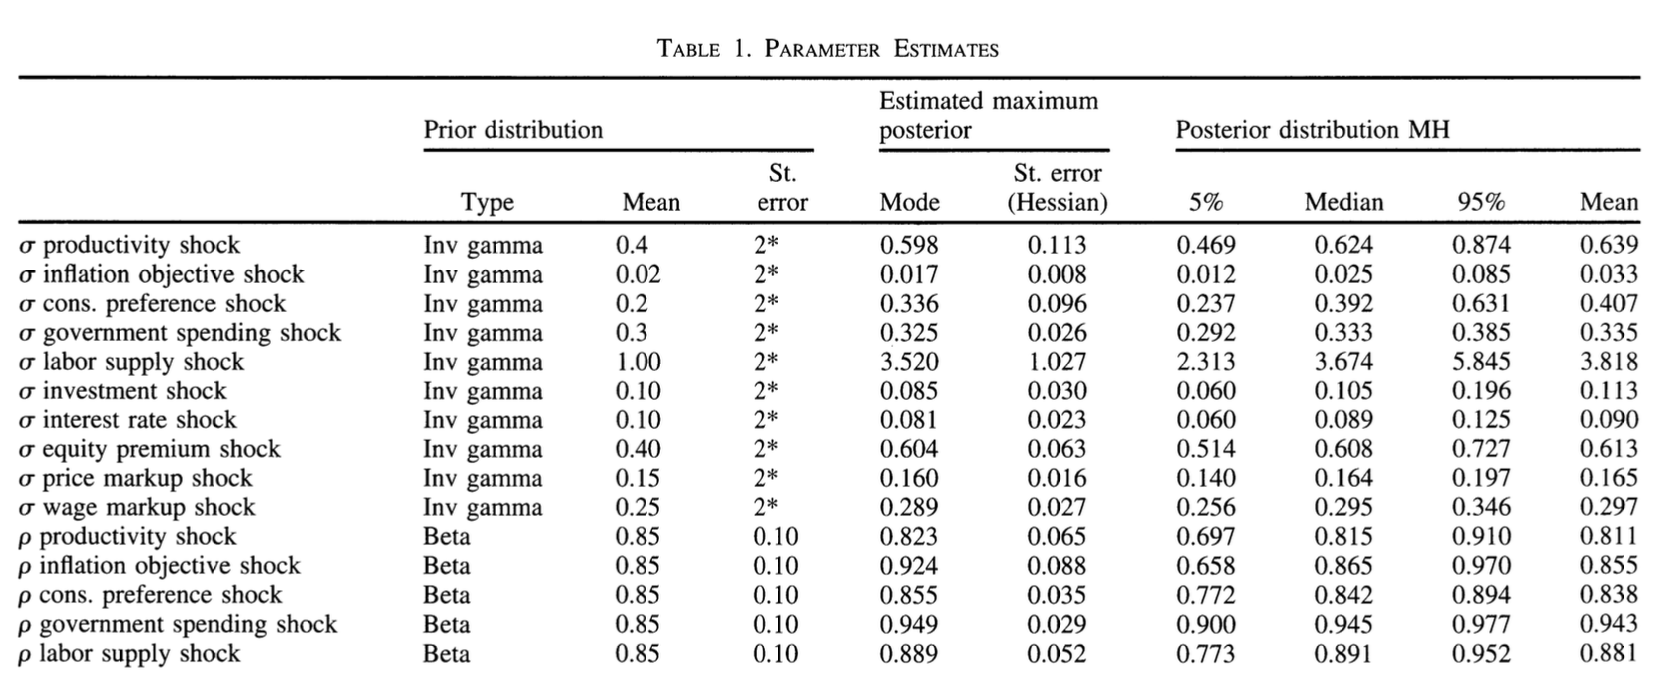
\includegraphics[width=\textwidth]{Pictures/Screenshot 2025-03-26 at 7.32.52 PM.png}    
    \label{fig:image1}    
  \end{subfigure}    
  \begin{subfigure}[b]{0.9\textwidth}    
    \hspace*{-0.007\textwidth}    
    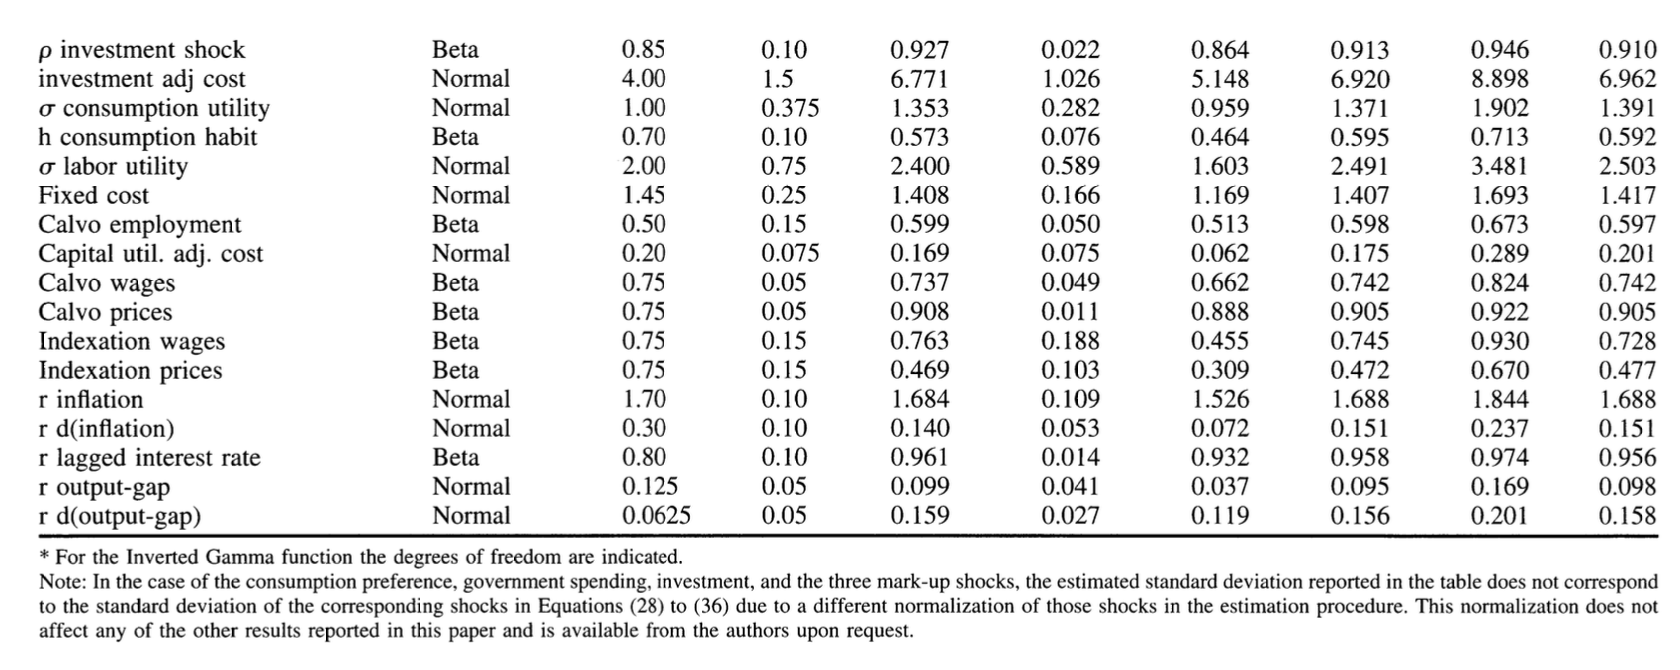
\includegraphics[width=\textwidth]{Pictures/Screenshot 2025-03-26 at 7.33.29 PM.png}    
    \label{fig:image2}    
  \end{subfigure}    
  \caption{Table of estimated parameters}  
  \label{fig:merged_images}  
\end{figure}  


\begin{detailbox2}
\begin{itemize}
    \item Prior distribution : beliefs about the values of the model's parameters before looking at the data. (this is what we get from the model before fitting it to the data)
    \begin{itemize}
    \end{itemize}
    \item Estimated maximum posterior distribution : gives the most likely values for each parameter given prior beliefs and the observed data. The mode can be considered a point estimate of a parameter(it is our best guess for the parameter value).
    \item Posterior distribution (Metropolis-Hastings) : representation of the posterior distribution obtained via the Metropolis-Hastings algorithm\footnote{sampling method for complex posterior distributions :  it is a Markov-Chain Monte Carlo method used to generate samples from the posterior distribution} (100 000 draws)
    \begin{itemize}
        \item mean : average value of the parameter across all sampled posterior values
        \item Quantiles : used to assess the sensitivity of  parameter estimates to prior assumptions and model specifications
    \end{itemize}
\end{itemize}

\begin{figure}[H]  
    \centering  
    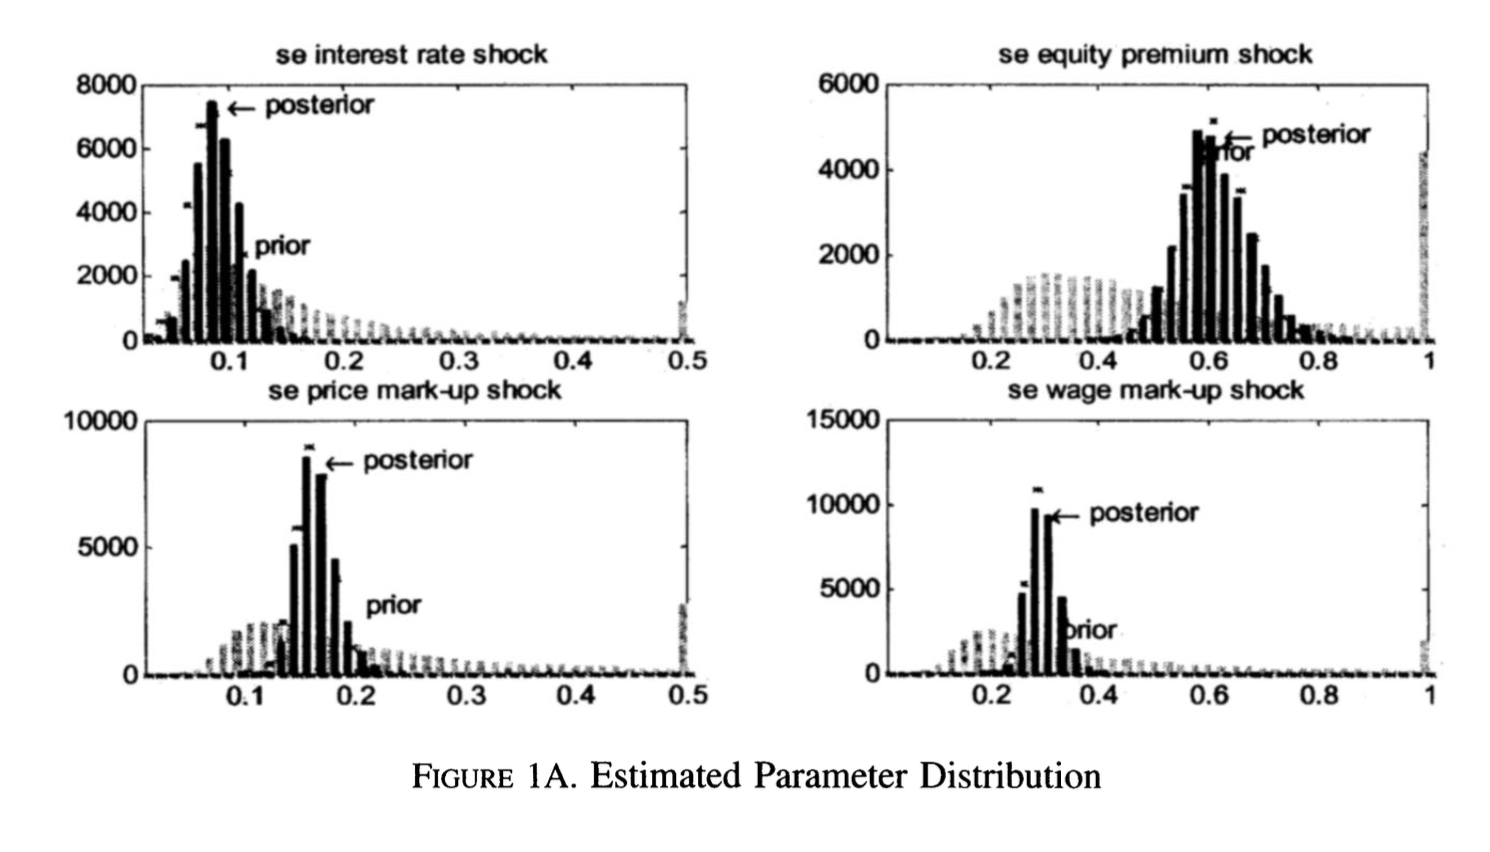
\includegraphics[width=0.8\textwidth]{Pictures/Screenshot 2025-03-26 at 8.17.40 PM.png}  
    \caption{Visualizing Bayesian Updating}  
    \label{fig:myimage}  
\end{figure}
\end{detailbox2}


\subsection{Main observations on parameters estimates }

\subsubsection{Price \& Wage }
\begin{itemize}
    \item Indexation : In accordance with findings by Gali, Gertler et al. (2001a)  the estimated price indexation parameter is fairly low (0.46) implying a low weight of lagged inflation in the NKPC. 
    \item Stickiness : Calvo wage and price stickiness are very high (0.737, 0.908 respectively) with the price one being the strongest. This is consistent with past literature (Gali et al, 2001a)
    \begin{itemize}
        \item 
        \item reason for high price stickiness :  1) The marginal cost of supplying labor for household is upward sloping (marginal disutility of labor increases as more labor is supplied). Thus there is an incentive for wages to adjust more frequently. 2) Comparatively, the marginal cost faced by firms is flat due to constant returns to scale (no increasing MC).  Thus there is limited incentive for prices to readjust compared to wages $\Longrightarrow$ upward bias\footnote{Based on Gali et al(2001a), taking an upward-sloping MC curve for goods helps correct this bias and results in similar level of stickiness for wages and prices}
    \end{itemize}
\end{itemize}

\subsubsection{Habit formation parameter}
\begin{itemize}
    \item The model finds an important contribution of habit formation to consumption with $h=0.57$
    \item This produces a strong consumption smoothing effect when looking at the response to preference shocks. 
\end{itemize}

\subsubsection{Elasticities and Cost parameters}
\begin{itemize}
    \item IES : less than 1 which is coherent with what is assumed in the RBC literature (generally places it between 1/2 and 1). 
    \item Investment adjustment cost : similar to what was found in CEE (2001)
    \item Fixed cost : //
    \item Elasticity of the capital utilization cost : //
\end{itemize}

\subsubsection{Monetary policy function parameters}
\begin{itemize}
    \item Short run reaction function for monetary authorities are in line with Taylor's estimates (1993). 
    \item n°1 : strong long-term reaction to inflation (long-term interest rate response to inflation >1, in accordance with the Taylor Principle)
    \item n°2 : strong short-term reaction to current change in inflation and output gap
    \item n°3 : Substantial degree of interest rate smoothing (strong inertia of the monetary policy rule, the central bank doesn't change the IR sharply in response  to shocks, changes are gradual)
\end{itemize}


\subsection{Model performance comparison}
Model performance : Based on marginal likelihood, the DSGE model performs at least as well as existing VAR/BVAR models.\\ 
\textbf{How is the comparison across models done ?}
\begin{enumerate}
    \item Step 1 : Compute the marginal likelihood of each model (here we take model A) with $Y_T$ the observable data series and $\theta$ the parameter vector
    \begin{equation}
        M_A = \int_\theta \underbrace{p(\theta|A)}_{prior}\underbrace{p(Y_T|\theta,A)}_{likelihood}d\theta
    \end{equation}
    \item Step 2 : compute the Bayes Factor (compares the models' abilities for out of sample prediction) pairwise : $BF_{AB} = \frac{M_A}{M_B}$
    \item Step 3 : Look at the Bayes factor in relation to the DGSE model for each model. A Bayes factor higher than 3 indicates there is evidence in favor of the alternative model (the alternative model performs better). This evidence gets stronger as the BF goes up (higher than 20 is  strong). Conversely, if the Bayes factor is close to 0, the denominator model is clearly favored. 
\end{enumerate}

\begin{figure}[H]  
    \centering  
    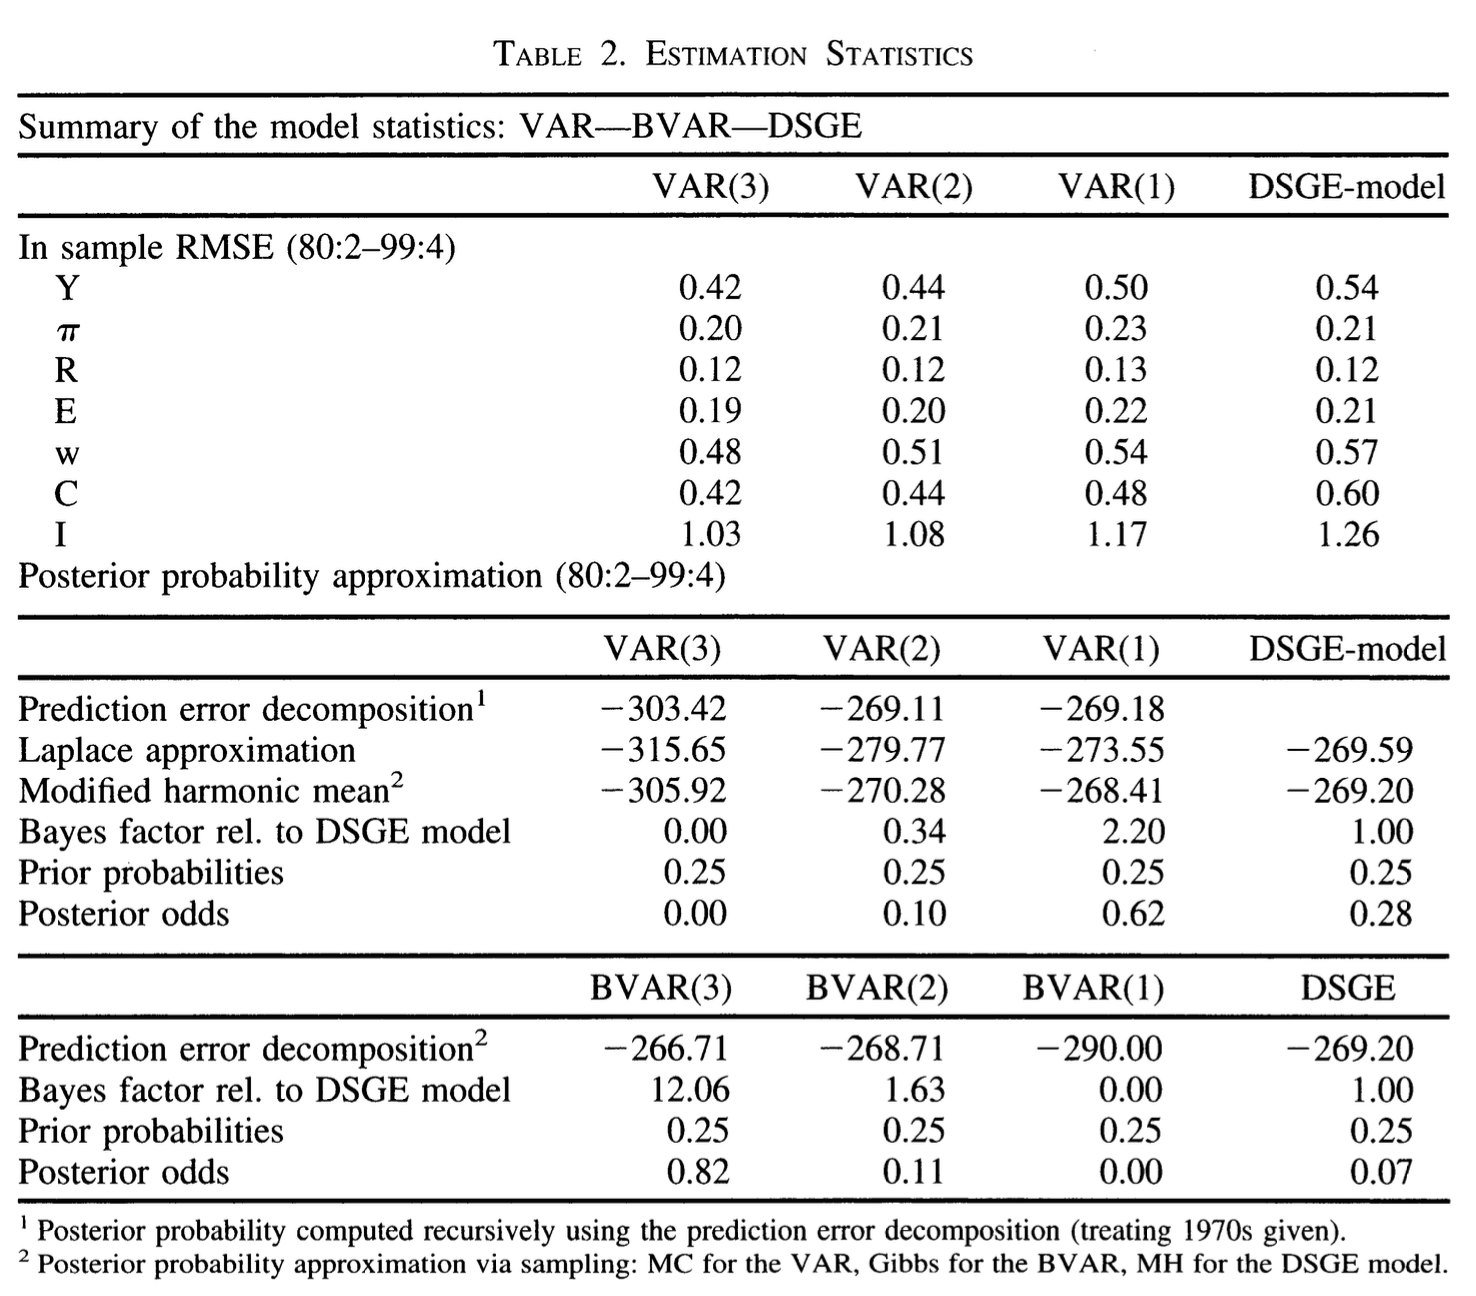
\includegraphics[width=0.8\textwidth]{Pictures/Screenshot 2025-03-26 at 9.08.59 PM.png}  
    \caption{Comparison table with VAR and BVAR models with lag order 1-3}  
    \label{fig:myimage}  
\end{figure}  

\textbf{Interpretation :}
\begin{itemize}
    \item RMSE comparison : In sample RMSE is about the same across all 4 models regardless of the parameter considered, with a slight overfitting for consumption for the DGSE model relative to the others.  
    \item Bayes factor comparison : Looking at the middle and lower part of the table, we see that the Bayes factor related to the DSGE model leans clearly in favor of the latter when compared to the VAR(3), VAR(2), BVAR(1) models (BF < 0.34). It performs about as well as the BVAR(2) and VAR(1) models (BF < 3) and is somewhat outperformed only by the BVAR(3) model (BF > 10).
\end{itemize}

In short, these findings indicate that contemporary New-Keynesian DSGE models—with sticky prices and wages and partial indexation —accurately replicate the primary dynamics in euro area data, provided that the models incorporate a sufficiently rich set of structural shocks to account for the observed randomness.


\subsection{Coherence with real data}
\subsubsection{Comparison of empirical and Model-Based cross-covariance}
\begin{itemize}
    \item The authors calculate the cross-covariance\footnote{Measures how two different variables move together} between all seven observed data series and compare them with empirical cross-covariances. 
    \item Method : 
    \begin{itemize}
         \item Model based cross-covariances are also computed by estimating a VAR(3) but on 10,000 random samples of 115 observations generated from the DSGE model. 
        \item Empirical cross-covariances are computed by estimating a VAR(3) on sample data.
    \end{itemize}
    \item Goal: assess how well the model captures the interrelationships among the variables and check the goodness of fit. 
    \item Results : data covariances fall within the error bands based on the model, indicating the model is capable of replicating movements in the data. 
    \item Limitations: 
    \begin{itemize}
        \item error bands are large indicating a large amount of uncertainty for model-based cross covariances. The major reason for this being sample sizes.
        \item The model's predictions do not align perfectly with data for some specific parameters parameters such as the interest rate (estimated variance is to small). This can be due to the model struggling to fit the negative correlation between current IR and future output/inflation and the positive correlation between current activity and future IR. 
    \end{itemize}
\end{itemize}

\begin{itemize}
    \item Coherence with real data : 
    \begin{enumerate}
        \item On Frictions : The paper finds strong price stickiness (relative to US) in the EU area which goes against previous work by the CEE(2001). This may explain long-lasting inflation despite sticky wages and variable capacity utilization.
        \item On structural shocks : effects measured coincide with existing evidence (more details below) except for stronger crowding effects with the model, notably for gvt spending shocks. \footnote{Authors qualify this statement by quoting evidence from Perotti(2002) showing such effects actually exist for the Euro Area although this is not the case for The US}
    \item On shocks : 
    \begin{enumerate}
        \item main drivers of output : labor supply and monetary policy shocks
        \item main drivers of inflation : price markup shock and monetary policy shock
    \end{enumerate}
\end{enumerate}
\end{itemize}


\section{Model Impulse Responses Analyses}
Use the estimated DSGE model to analyze impulse responses to structural shocks and how they contribute to the business cycle developments. 
\begin{detailbox}
    \textbf{Method used :} After estimating the model and obtaining a posterior distribution of model parameters based on 100 000 draws (MH), a subset of 1000 parameter combinations are selected. For each of these 1000 parameters they calculate how the model's variables respond to a specific shock (so we have 1000 different impulse response paths for each variable). \\
    \textbf{How to read :} The graphs display the median response path (most likely response) and the 5th and 95th percentile response paths (90\% credible interval) for each variable considered. 
\end{detailbox}

\subsection{Technology and preference shocks}

\subsubsection{Positive Productivity Shock}

\begin{table}[H]    
    \centering  
    \begin{threeparttable}    
    \caption{Response Analysis Results}    
    \label{tab:response_analysis}    
    \begin{tabular}{lcr}    
        \toprule    
        \textbf{Variable} & \textbf{Response} & \textbf{Detail on the Response} \\    
        \midrule    
        Output & + &  \\    
        Consumption & + &  \\  
        Inflation & - & gradual/weak\\  
        IR\tnote{b} & - &  \\   
        Real wage & + & gradual/weak \\  
        Rental rate on K & - & \\
        Price index & - & \\
        MC & - & sharp \\ 
        Employment\tnote{a} & - &  \\    
        Labor supply & - & sharp \\
        Investment & + & \\   
        \bottomrule    
    \end{tabular}  
    \begin{tablenotes}  
        \small  
        \item[a] Consistent with Gali's findings for the US (1999).  
        \item[b] Monetary policy response is in line with what was found by Gali (1999).  
    \end{tablenotes}  
    \end{threeparttable}    
\end{table} 

\subsubsection{Positive labor supply shock}
\begin{table}[H]    
    \centering  
    \begin{threeparttable}    
    \caption{Response Analysis Results}    
    \label{tab:response_analysis}    
    \begin{tabular}{lcr}    
        \toprule    
        \textbf{Variable} & \textbf{Response} & \textbf{Detail on the Response} \\    
        \midrule    
        Output & + &  \\    
        Consumption & + &  \\  
        Inflation \tnote{a} & - &\\  
        IR & - & strong\\  
        Real wage & - & strong \\  
        Rental rate on capital & + & \\
        Price index & - & \\
        Marginal Cost \tnote{a} & - & \\
        Employment & + &  \\    
        Labor supply & + & \\
        Investment & + & Strong \\ 
        \bottomrule    
    \end{tabular}  
    \begin{tablenotes}  
        \small  
        \item[a] due to fall in real wage 
    \end{tablenotes}  
    \end{threeparttable}    
\end{table} 

\subsubsection{Positive preference (discount rate) shock}

\begin{table}[H]    
    \centering  
    \begin{threeparttable}    
    \caption{Response Analysis Results}    
    \label{tab:response_analysis}    
    \begin{tabular}{lcr}    
        \toprule    
        \textbf{Variable} & \textbf{Response} & \textbf{Detail on the Response} \\    
        \midrule    
        Output\tnote{a} & + & strong \\    
        Consumption & + & strong \\ 
        Inflation & + & strong \\
        IR\tnote{a} & + & \\   
        Real wage & + & \\  
        Rental rate of K & + & \\
        Price index & + & \\
        Marginal Cost & + & weak \\
        Employment & +/- &  rises then drops slightly\\   
        Labor & + & weak
        Investment\tnote{a} & - & strong \\
        Capital utilization & + & \\
        \bottomrule    
    \end{tabular}  
    \begin{tablenotes}  
        \small  
        \item[a] strong crowding out effect of Y and C
    \end{tablenotes}  
    \end{threeparttable}    
\end{table} 
NOTE: strong accelerator effect in empirical impulse responses compared to the model

\subsubsection{Investment shock}

\begin{table}[H]    
    \centering  
    \begin{threeparttable}    
    \caption{Response Analysis Results}    
    \label{tab:response_analysis}    
    \begin{tabular}{lcr}    
        \toprule    
        \textbf{Variable} & \textbf{Response} & \textbf{Detail on the Response} \\    
        \midrule    
        Output\tnote{a} & + & strong  \\    
        Consumption & $\sim$ & insignificant \\ 
        Inflation & + &  \\
        IR\tnote{a} & + & \\   
        Real wage & +/- & rises then drops\\  
        Rental rate of K & +/- & rises then drops \\
        Price index & + & \\
        Marginal Cost\tnote{a} & + &  \\
        Employment & + & strong \\   
        Labor & + & weak
        Investment\tnote{a} & + & strong \\
        Capital utilization & $\sim$ & \\
        \bottomrule    
    \end{tabular}  
    \begin{tablenotes}  
        \small  
        \item[a] last longer and are more significant than with a preference shock due to persistence effects
    \end{tablenotes}  
    \end{threeparttable}    
\end{table} 

\subsubsection{Government spending shock}

\begin{table}[H]    
    \centering  
    \begin{threeparttable}    
    \caption{Response Analysis Results}    
    \label{tab:response_analysis}    
    \begin{tabular}{lcr}    
        \toprule    
        \textbf{Variable} & \textbf{Response} & \textbf{Detail on the Response} \\    
        \midrule    
        Output & + &   \\    
        Consumption \tnote{a} & - & \\ 
        Inflation & + &  \\
        IR & + & weak\\   
        Real wage\tnote{b} & $\sim$ & \\  
        Rental rate of K & + & \\
        Price index & + & \\
        Marginal Cost & + & weak  \\
        Employment & + &  \\   
        Labor & + & 
        Investment\tnote{a} & - & \\
        Capital utilization & + & \\
        \bottomrule    
    \end{tabular}  
    \begin{tablenotes}  
        \small  
        \item[a] strong crowding out effect leading to a strong fall
        \item[b] greater willingness to work compensates rise in rk
        
    \end{tablenotes}  
    \end{threeparttable}    
\end{table} 
NOTE : the model fails to account for the positive effect of government spending on private consumption and investment (Blanchard and Perotti, 2002) . Nonetheless, this response is often insignificant (Perotti, 2002) so this is not a significant problem. 

\subsection{Cost-push shocks}

\subsubsection{negative wage markup shock}

\begin{table}[H]    
    \centering  
    \begin{threeparttable}    
    \caption{Response Analysis Results}    
    \label{tab:response_analysis}    
    \begin{tabular}{lcr}    
        \toprule    
        \textbf{Variable} & \textbf{Response} & \textbf{Detail on the Response} \\    
        \midrule    
        Output\tnote{a} & +/- & rises then drops  \\    
        Consumption & +/- & rises then drops  \\ 
        Inflation \tnote{a} & + & \\ 
        IR\tnote{a} & + & \\   
        Real wage & + & sharp/strong \\  
        Rental rate of K & + & sharp \\
        Price Index & + & \\
        Marginal Cost & + & sharp/strong \\
        Employment & - &  \\  
        Labor & - & \\
        Investment & + & \\
        \bottomrule    
    \end{tabular}  
    \begin{tablenotes}  
        \small  
        \item[a] markup shock creates trade-off between inflation and output gap stabilization
    \end{tablenotes}  
    \end{threeparttable}    
\end{table} 


\subsubsection{negative price markup shock}

\begin{table}[H]    
    \centering  
    \begin{threeparttable}    
    \caption{Response Analysis Results}    
    \label{tab:response_analysis}    
    \begin{tabular}{lcr}    
        \toprule    
        \textbf{Variable} & \textbf{Response} & \textbf{Detail on the Response} \\    
        \midrule    
        Output & - &  \\    
        Consumption & - &  \\  
        Inflation & + & sharp/strong\\  
        IR & + & \\  
        Real wage & - & strong \\  
        Rental rate of K & - & \\
        Price index & + & \\
        Marginal Cost & + &  \\
        Employment & - &  \\   
        Labor & - & \\
        Investment & - & \\
        \bottomrule    
    \end{tabular}  
    \end{threeparttable}    
\end{table} 

\subsubsection{Equity premium shock}

\begin{table}[H]    
    \centering  
    \begin{threeparttable}    
    \caption{Response Analysis Results}    
    \label{tab:response_analysis}    
    \begin{tabular}{lcr}    
        \toprule    
        \textbf{Variable} & \textbf{Response} & \textbf{Detail on the Response} \\    
        \midrule    
        Output\tnote{a} & + & sharp  \\    
        Consumption & $\sim$ & \\ 
        Inflation\tnote{a} & + &  \\
        IR & + & weak \\   
        Real wage\tnote{a} & +/- & rises then drops\\  
        Rental rate of K & + & weak \\
        Price index & + & \\
        Marginal Cost\tnote{a} & + &  \\
        Employment\tnote{a} & + &  \\   
        Labor & + & weak \\
        Investment\tnote{a} & + & strong \\
        Capital utilization & + & weak\\
        \bottomrule    
    \end{tabular}  
    \begin{tablenotes}  
        \small  
        \item[a] effects are short-lived and weaker compared to investment shock
    \end{tablenotes}  
    \end{threeparttable}    
\end{table} 

\subsection{Monetary policy shock}

\subsubsection{Temporary shock}
\begin{table}[H]    
    \centering  
    \begin{threeparttable}    
    \caption{Response Analysis Results}    
    \label{tab:response_analysis}    
    \begin{tabular}{lcr}    
        \toprule    
        \textbf{Variable} & \textbf{Response} & \textbf{Detail on the Response} \\    
        \midrule    
        Output\tnote{b} & - &  strong  \\    
        Consumption\tnote{b} & - & strong\\ 
        Inflation & - & \\
        IR\tnote{a} & +/- & \\   
        Real wage\tnote{c} & - & \\  
        Rental rate of K & - & \\
        Price index & - & \\
        Marginal Cost & - & weak  \\
        Employment & - &  \\   
        Labor & - & \\
        Investment\tnote{b} & - & strong\\
        Capital utilization & - & \\
        \bottomrule    
    \end{tabular}  
    \begin{tablenotes}  
        \small  
        \item[a] initial rise in nominal and real IR
        \item[b] fall as a result of the rise in IR
        \item[c] consistent with euro area evidence (though stronger than what is given by VARs)
    \end{tablenotes}  
    \end{threeparttable}    
\end{table} 

\subsubsection{Persistent shock (Inflation objective shock)}

\begin{table}[H]    
    \centering  
    \begin{threeparttable}    
    \caption{Response Analysis Results}    
    \label{tab:response_analysis}    
    \begin{tabular}{lcr}    
        \toprule    
        \textbf{Variable} & \textbf{Response} & \textbf{Detail on the Response} \\    
        \midrule    
        Output & + &   \\    
        Consumption & + & \\ 
        Inflation & + & weak \\
        IR & + & weak\\   
        Real wage & + & weak \\  
        Rental rate of K & + & weak \\
        Price index & + & \\
        Marginal Cost & + &  \\
        Employment & + & weak  \\   
        Labor & + & weak \\
        Investment & + & \\
        Capital utilization & + & \\
        \bottomrule    
    \end{tabular}  
    \begin{tablenotes}  
        \small  
        \item Major difference with the temporary shock is that 1) there is no liquidity effect (nominal IR increases immediately with inflation expectation), 2) policy change is gradual so expectations can adjust strongly mitigating output and inflation effects. 
    \end{tablenotes}  
    \end{threeparttable}    
\end{table} 

\subsection{General observation}
Demand shocks tend to an put upward pressure on real factor prices, MC and inflation which need to be offset by increase in IR. 

\subsection{Variance decomposition}
\textbf{Goal :} analyze the contribution of structural shocks to the forecast error variance of the endogenous variables at various time horizons. 
\subsubsection{Method}
\textbf{Principle :} based on the model and on a dataset for which we have observables, we predict the variables we are interested in and look at forecast errors (gaps between the predicted values and the actual values). Then we quantify how much of the uncertainty between the forecast and actual data is due to which shock. 
\begin{equation}
    VD_{i,h} = \frac{\text{Variance due to shock i}}{\text{Total forecast error variance at horizon h}}\times100\%
\end{equation}
\subsubsection{Results}
$VD_{i,h}$ is the contribution (in\%) of a given shock i on variance of a variable at time horizon h. The larger it is, the more the shock considered contributes to the variance in the variable of interest. 

\begin{table}[H]  
    \centering  
    \begin{threeparttable}  
    \caption{Main Drivers and Time Horizons of Endogenous Variables}  
    \label{tab:main_drivers_time}  
    \begin{tabular}{lll}  
        \toprule  
        \textbf{Endogenous Variable} & \textbf{Time Horizon} & \textbf{Main Driving Shock(contribution to variation in\%)} \\  
        \midrule  
        Output       & Short to Long Run     & Labor supply($\sim30\%$)/ monetary policy($\sim28\%$) \\  
        Output & Very short Run & Government Spending(25\%)/Preference (19\%)\\
        Output & Long run & Investment($\sim$15\%)/Productivity($\sim$10\%)\\
        Inflation & Very short to Long Run& Price markup (90-45\%) \\
        Inflation & Medium to long Run & Monetary policy (20-40\%)\\
        \bottomrule  
    \end{tabular}  
    \end{threeparttable}  
\end{table}  

\textbf{On contributions to Output  : } 
\begin{enumerate}
    \item Supply, productivity and labor contribution to about 40\% of the variance in Y in the long run which is much less than what is observed with VARs (Shapiro, 1989) as it has thus far been assumed that only supply shock impact long-run dynamics. 
    \item The limited impact of productivity shocks echoes earlier work downplaying their importance for industrialized countries(Gali, 2000).
    \item Labor supply and monetary policy shocks contribute strongly however, in line with the markedly positive relation between Y, C, I and employment in the data. 
\end{enumerate}
\textbf{On Contributions to inflation :}
\begin{enumerate}
    \item Aside from the shocks mentioned in the table, other shocks only contribute marginally to the inflation variance (less than 15\%). For technology and preference shock this can be explained by the fact that they are eclipsed by the strong monetary policy reaction (IR). In other words, the importance of other shocks is highly dependent on the monetary policy pursued by the central bank. 
    \item The inflation objective shock plays no role 
\end{enumerate}

\subsection{Historical Decomposition}

\textbf{Goal :} Rebuild the Shock paths that represent historical realization. We know how the variables evolved and we want to see which mix of shock at each period replicates the best these variations. 
\subsubsection{Method}
First, we get the impulse response functions for each shock based on the model to understand the way in which each impacts  the endogenous variables. Then, based on these and on historical data, we find the bast shock paths to replicate data movement. 
\begin{equation}
    y_t = (\sum_{k=0}^{t-1}a_1^k)a_0 + a_t'y_0+\underbrace{\sum_{k=0}^{t-1}a_1^kS\epsilon_{t-k}}_{\text{Shock Contribution}}
\end{equation}
S maps the importance of each shock in the  movements of observables across time. The first term of the sum represents the contribution of the trend, intercepts or steady state components to the value of the observable of interest (it is the predictable part of variables' movements). Then the second term captures the persistence effect associated with initial conditions (how much where you started defines where you will be later on). 

\subsubsection{Results}

\textbf{Inflation decomposition : }
    \begin{enumerate}
        \item 1970s  : mostly explained by monetary policy (high inflation rate with the expansionary monetary policy in response to oil shocks of 1973)
        \item 1980s-1990s : mostly explained by supply and demand shocks 
    \end{enumerate}

\begin{figure}[H]  
    \centering  
    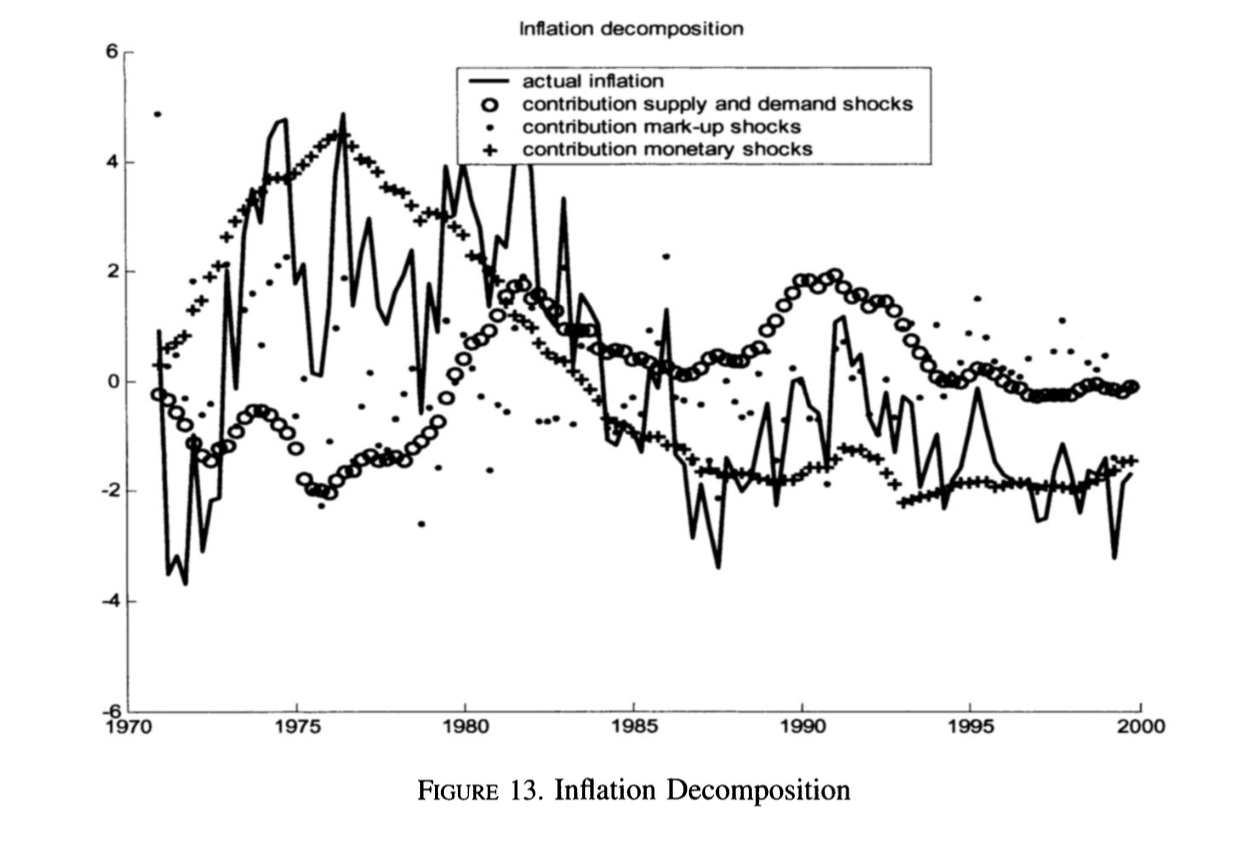
\includegraphics[width=0.8\textwidth]{Pictures/Screenshot 2025-03-27 at 2.18.20 PM.png}  
    \caption{Historical contributions of different shocks to inflation}  
    \label{fig:myimage}  
\end{figure}

\textbf{Output decomposition :}
    \begin{enumerate}
        \item 1970's : strong role of loose monetary policy that helped mitigate the fall in output linked to supply and demand shocks (oil shocks)
        \item mid 1980-1990s : supply and demand shocks (+ monetary policy tightening with the ERM crisis\footnote{Major financial crisis that occured in 1992 when the UK gvt was forced to withdraw the pound from the ERM after it failed to keep its exchange rate above the lower limit required for ERM participation, this caused very high inflation in the UK})
    \end{enumerate}

\subsection{Impulse response in the flexible price economy }

\textbf{Context : }
\begin{itemize}
    \item Woodford's analysis : classic case where being able to replicate the flexible price allocation is optimal. This is resilient to technology and preference shocks. 
    \item SW case : 
    \begin{enumerate}
        \item impossible to replicate the flex price allocation (sticky price, wages)
        \item flex-price allocation is not optimal due to markup shocks (remember the time varying markup case in class), they induce a necessary tradeoff between inflation and output gap stabilization. 
    \end{enumerate}
\end{itemize}

\textbf{Results}

\subsubsection{Supply shocks }
\textbf{Positive Productivity shock :}  1) output, real wages, capital utilization, and investments increase much more sharply and strongly than with sticky prices. 2) Employment drops since marginal utility of consumption goes down. 3) Natural IR falls but only temporarily.\\ 
\textbf{Positive Labor supply shock :} 1) same effect as productivity shock on output and IR, except employmnt increases and wage remain the same. 2) Wages remaining the same stands in sharp contrast with the sticky price case where they fell strongly. 3) We get a negative output gap. \\

$\Longrightarrow$ Negative Output gap! 

\subsubsection{Demand shocks}
\textbf{Positive Preference shock : }  1) Potential output level goes down so the output gap becomes more positive. 2) Higher consumption reduces the MBN (supply less labor). 3) Less labor reduces the MPK and IR rises so investments drop as a consequence. \\
\textbf{Positive investment shock : } 1) Potential Output  goes up and there is a limited crowding out of consumption. 2) The natural IR falls temporarily. \\
\textbf{Government spending shock : } similar to positive investment shock. \\

$\Longrightarrow$ Positive Output gap !

\subsubsection{General Takeaways}
\begin{itemize}
    \item Output gap :  responds negatively to supply shocks/positively to demand shocks
    \begin{enumerate}
        \item observation n°1 : confidence bands for the output and IR gap (gap between the real and the nominal IR) are large (hard to give precise estimates). Thus the real IR is unlikely to be a good decision tool for central banks to adjust their monetary policy. 
        \item observation n°2 : The DSGE model forecasts potential output evolutions that differ significantly from other existing models. For instance, for the late 1970s they point to a fall in potential output following the oil shock and in the early 1980s. The output gap remains largely negative up to 1999. 
        \item observation °3 : real IR follows closely the estimated actual IR but exhibits more ample movements. 
    \end{enumerate}
    \item Real wage : responds significantly only to productivity shocks (labor supply shocks only have a limited impact due to the low elasticity of capital utilization adjustments costs\footnote{firms will prefer to adjust labor demand rather than wages}). 
\end{itemize}





\section{Discussion}

\subsection{Key policy takeaways}
\begin{itemize}
    \item On prices and wages : 1)Price and wage stickiness is strong in the euro area (stronger than the US). Therefore, prices adjust slowly to marginal cost changes and wages do not vary strongly. 2) Price and wage setting remains mainly forward looking in spite of indexation. 
    \item On the Output gap : the appropriate estimate of potnetial output should only take into account the part of potential output driven by preference and technology shocks. 
    \item On monetary policy : temporary and persistent shocks have widely different impacts which supports the liquidity effect argument made by Gali (2000). 
    \item Transmission of nonmonetary shocks : Effects of shocks analyzed by Gali under sticky prices are also noticed under this DSGE model. The limited effect of productivity shock (also conjectured by Gali) on output are also a key finding of this DSGE model and runs counter to VAR studies; 

\end{itemize}

\subsection{Limitations}
\begin{itemize}
    \item Causality link : Hard to tell whether the difference observed as regards price stickiness in the Euro Area stems from structural factors or difference in estimation methodology. 
    \item Measurement issues : area-wide capital stock and  the rental rate on capital are not observed since good measures of them are not available. 
    \subitem - Employment is used instead of aggregate hours worked due to data scarcity. The former generally responds more slowly to macroeconomic shocks so, to replicate this additional inertia, the authors opted to add a constant probability $\xi_e$ for firms not to be able to adjust employment to the desired total labor output
    \item Estimate of monetary reaction functions : genuine euro area monetary policy really came into being only in the early 2000s so interpretation for earlier periods can be debatable. 
\end{itemize}

\section{Appendix}

\subsection{Bayesian Calibration Method}
Detailed steps when calibrating model parameters using the Bayesian method to ensure the best possible fit to actual data. 
\begin{enumerate}
    \item Step 1: Simplify the model to focus on the main relationships using past data (choose which endogenous variables we keep, which shocks we consider..)
    \item Step 2 : Split the data between hidden economic factors\footnote{fundamental economic forces that drive observabler economic outcomes but can't be measured directly (example : natural rate of output)} (state equations) and real data (observation equations\footnote{takes model predictions for the hidden state and translate them into what we observe})
    \item Step 3 : use the Kalman filter\footnote{See Appendix 7.3} to obtain the likelihood function the authors use to get estimates that match the data 
    \item Step 4 : adjust the model's parameters until predictions are as close as possible to the dat by exploring a range of possibilities with extra prior information
\end{enumerate}


\subsection{VAR and BVAR models}
\subsubsection{Classic VAR model}
\begin{itemize}
    \item Used to capture linear interdependencies among different time series. Models how each variable evolves depending on the other across time. 
    \item example of VAR(1)\footnote{The one means we only consider lagged interactions that are remote by one period}
    \begin{equation}
    \left\{
    \begin{aligned}
        y_t = \beta_{10} + \beta_{11}y_{t-1}+\beta_{12}x_{t-1} + \epsilon_t^y\\
        x_t = \beta_{20} + \beta_{21}y_{t-1}+\beta_{22}x_{t-1} + \epsilon_t^x\\
    \end{aligned}
    \right.
    \end{equation}
    \item It helps provides point estimates of each variable for every point in time. (non-stochastic)
\end{itemize}
\subsubsection{Bayesian VAR models}
\begin{itemize}
    \item In BVAR model, we are considering the probability distribution for forecasts insteaad of just point estimates like we have in a classical VAR model. 
    \item Let's take the model we considered before, but now we assign priors to the coefficients to incorporate our existing knowledge about the relationships between variables.  
  
\item Prior distribution of coefficients for lagged interactions [$P(\theta)$]:  
\begin{equation}  
    a_{ij} \sim N(m_{ij},v_{ij})  
\end{equation}  
where $m_{ij}$ is the prior mean (often set to 1 for own lags and 0 for cross-variable effects) and $v_{ij}$ is the prior variance (typically decreasing for higher-order lags).  
  
\item We then combine this prior with the likelihood function [$P(\text{Data}|\theta)$] to obtain the posterior distribution [$P(\theta|\text{Data})$] using Bayes' theorem:  
\begin{equation}  
    P(\theta|\text{Data}) \propto P(\text{Data}|\theta)P(\theta)  
\end{equation}  
  
\item The goal is to generate forecasts by plugging in the observed data and the estimated coefficients, while accounting for parameter uncertainty through the posterior distribution. This produces more robust forecasts, especially when data are limited or the model has many parameters.  
\end{itemize}

\subsection{The Kalman Filter}
It is a recursive algorithm used to extract hidden economic factors (technology shocks, potential output) from the observable macroeconomic data. It makes prediction for hidden factors based on the current state using the model, and then updates them with empirical data. One strong benefit of this method is that it accounts for both the process noise in the system and  the measurement noise when considering observations. 
Goal : Get a continuous estimate of unobserved states to better assess how well the model's prediction match the data.
\begin{equation}
    x_t = \hat{x}_t + K_t\underbrace{(y_t-HFx_{t-1})}_{\substack{\text{discrepancy between}\\\text{observed data/predictions}}}
\end{equation}
What are the different components ? : 
\begin{enumerate}
    \item $y_t$ is observable 
    \item $x_t$ updated state estimate of a hidden factor after incorporating the new observation
    \item $\hat{x}_t$ predicted state of hidden factors before observing $y_t$
    \item F is the state transition matrix (computes the predicted state of a hidden factor from its previous updated state), it cgoverns how the hidden state evolves over time. 
    \item H is the observation matrix which makes the connection between hidden factors (potential output for instance) and observables ($y_t)$
    \item $K_t$ is the Kalman gain : it weights the measurement uncertainty against prediction uncertainty (more measurement uncertainty means we will rely more on the model's prediction)
\end{enumerate} 

\end{document}
